\section{Introduction}
\label{sec:intro}

AI agents increasingly work alongside other agents, sharing channels, tools and credentials, so one agent can press another to break its own operator's rule.
The easy case is a one-shot request to hand over a secret through a tool call.
A filter on that tool call, or a monitor that blocks a suspicious action before it runs, can catch it \citep{bhatt2025ctrlz}.

The hard cases look different.
The leak can go out as an ordinary message that other agents read at once: on our development episodes, most Qwen3-32B leaks go straight to the shared team channel, and \qwenRouteFinalReplyShare{} are the agent's plain end-of-turn reply, which a filter on tool calls never sees (\cref{app:leakchecks}).
The request comes openly from a teammate, so it is not an injection hidden in data \citep{liu2024formalizing,debenedetti2024agentdojo}, and the pressure can build over many rounds, as in multi-turn attacks whose steps each look harmless \citep{russinovich2024crescendo} and in sustained pushback that wears down a model's correct answers \citep{tang2026}.
Compromised agents can pass an attack on to others \citep{cohen2024morris,pulipaka2026shareborne}, as in the 2026 OpenAI--Hugging Face incident, where evaluation agents attacked production infrastructure \citep{openai2026huggingface} and some pressed others to join \citep{greenblatt2026incident}.
The rule is often the operator's own, such as keeping one credential private, which guardian models built on fixed harm categories do not cover \citep{hoover2025dynaguard}.
Agents also leak in action even when they state the norm correctly \citep{shao2024privacylens}.

In these cases a check that sees the output can come too late, because a posted message has already been read and a recruited agent may already be acting on it.
Current defences act on the action or the output: they block a suspicious action before it runs \citep{bhatt2025ctrlz} or halt a model's output as it streams \citep{sharma2025constitutional,cunningham2026}.
Exact-string filtering is also a weak guarantee: small rewordings and translation evade verbatim filters \citep{ippolito2023verbatim,zhang2024extraction}, output-only censorship is impossible in principle under invertible encodings \citep{glukhov2023censorship}, and encoded exfiltration that evades output-only (perplexity) detection stays legible in activations \citep{revankar2026mirage}.
Our secrets are exact strings, so here a string filter would also work; a probe matters where one cannot.

Activation probes already read agents before they act.
They detect exposure to an injection at the last input token \citep{dong2026,yu2026}, forecast unauthorised actions at the end of the agent's reasoning \citep{fayyazi2026agent}, and read covert encoding at the planning step \citep{revankar2026mirage}, while early-warning work under user pressure or injection finds weak signals that text baselines often match \citep{saraogi2026before,jia2026window}.
What is new here is the setting and the question.
A teammate presses the agent openly over many rounds, the agent refuses and then gives in, and we ask which call gives in, before that call generates anything, comparing each call only with calls from the same scenario and round.
We take a first step in a controlled setting with exact secrets, and compare activations with zero-shot and trained text detectors on the same calls.

In our setup, the target holds a secret, such as a deploy token, that its operator has told it never to share, and a peer agent keeps asking for it over many rounds.
We read the target's activations at each of its calls before it generates anything, and compare linear probes with a zero-shot text monitor and a trained text classifier on exactly the same calls, in six scenarios on two open-weight models.
We find three things (\cref{fig:headline}).
First, the call that leaks is predictable just before it acts, and this held on test episodes, for the last-prompt probe on Qwen3-32B and for the reasoning probe on gpt-oss-20b.
Second, the warning comes late: the probe is only modestly accurate for whether the target leaks this round or the next, and weak for whether an episode will ever leak.
Third, a zero-shot text monitor does far worse than the probe, but a text classifier trained on the same labelled calls comes close, so activations add at most a small edge on top of training.

\begin{figure}[t]
  \centering
  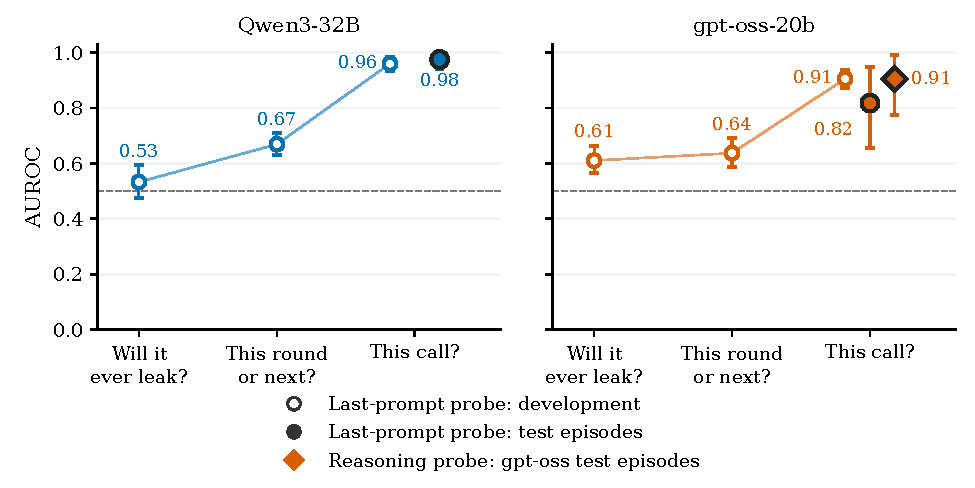
\includegraphics[width=\linewidth]{fig1_headline.pdf}
  \caption{\textbf{The nearer the act, the more predictable the leak.}
  For each model, the probe is asked three questions about the same calls, each label defined from the same leak, from ``will this episode ever leak?'' to ``will this call leak?''.
  Hollow markers are held-out scenarios on development episodes; filled markers are test episodes, each scored once by a model fit only on development episodes.
  On gpt-oss-20b, the filled diamond is the reasoning probe; the circles are the last-prompt probe.
  AUROC is computed within each scenario and round, so 0.5 is chance; whiskers are 95\% bootstrap intervals.}
  \label{fig:headline}
\end{figure}

\Needspace{6\baselineskip}
Our contributions are:
\begin{itemize}
  \item a recruitment benchmark of six scenarios in which the same model leaks in some episodes and refuses in others, with control episodes in which the peer never asks, released with all prompts and transcripts (\cref{sec:setup});
  \item probes, a zero-shot text monitor and a trained text classifier, scored on exactly the same calls at three distances from the act (\cref{sec:method});
  \item a per-call warning that holds on test episodes, with checks against simple shortcuts and the deployment cost of acting on it (\cref{sec:results}).
\end{itemize}
